\subsection{Refinement of Symbolic Value Analysis + ConstraintsCPA}

\begin{figure}[h!]
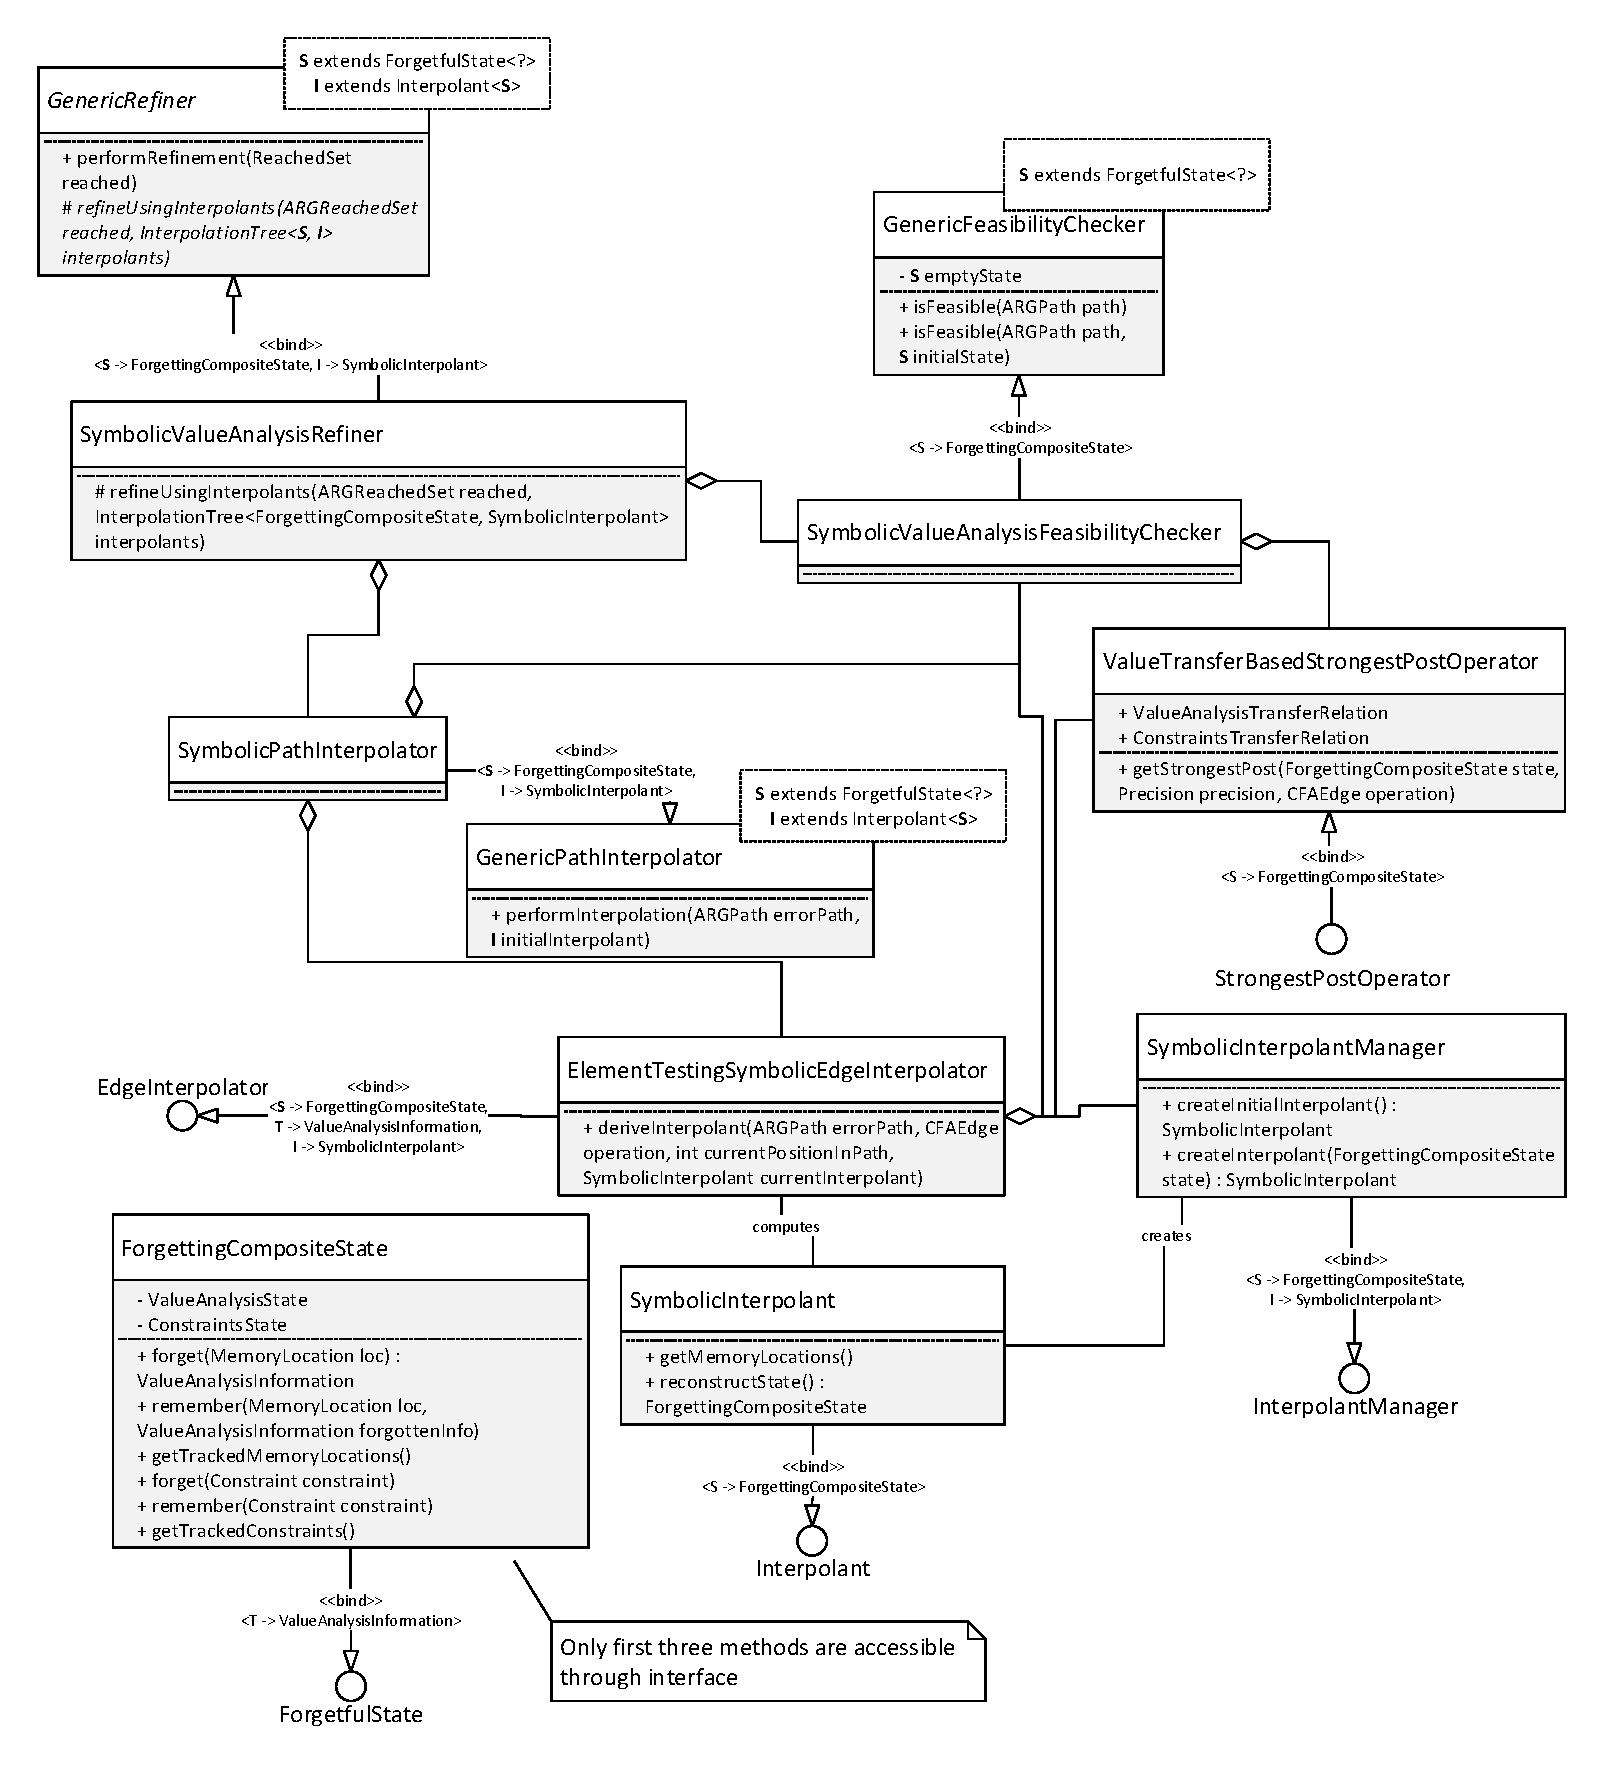
\includegraphics[width=1.2\linewidth]{implementationCegar/RefinementSymEx}
\caption{Structure of refinement procedure for symbolic execution}
\label{fig:refSymbolic}
\end{figure}
Refinement of the \symbolicValueAnalysisCPA\ and \constraintsCPA\ is strongly based on these generic implementations.
Besides \objectName{Interpolant}, \objectName{ForgetfulState}, \objectName{InterpolantManager} and \objectName{StrongestPostOperator}, we only
create an own implementation of \objectName{EdgeInterpolator}.
For all other components, we inherit the behaviour of the generic implementations.
Figure~\ref{fig:refSymbolic} shows the structure of this refinement.

\objectName{Sym\-bo\-lic\-Inter\-po\-lant} implements \objectName{Interpolant}.
It stores information about abstract variable assignments and constraints, so it can be used for interpolating over both these types.
\objectName{Forget\-ting\-Com\-po\-site\-State} implements \objectName{ForgetfulState}.
It is the composition of \objectName{ValueAnalysisState} and \objectName{ConstraintsState} and provides methods for forgetting/remembering both their elements separately.
This is necessary for interpolation, described below.
\objectName{SymbolicInterpolantManager} is an \objectName{InterpolantManager} able to create \objectName{SymbolicInterpolants}.
\objectName{Value\-Trans\-fer\-Based\-Strong\-est\-Post\-Operator} is the implementation of the composite strongest-post operator using the value analysis transfer relation and constraints transfer relation,
described in Section~\ref{sec:assignmentRefinement}.

\objectName{Sym\-bo\-lic\-Edge\-Inter\-po\-lator} implements \objectName{EdgeInterpolator}.
We can't use the functionality of \objectName{Generic\-Edge\-Inter\-po\-lator} since, depending on the configuration, we have to interpolate
testing both constraints and/or variable assignments for their necessity.
The generic edge interpolator only tests program variables (\objectName{Me\-mo\-ry\-Lo\-cations}), though.

%\subsubsection{Optimization: Perform basic Value Analysis refinement first}


\subsubsection{Extract precision from predicate refinement}
